% Template for ICASSP-2020 paper; to be used with:
%          spconf.sty  - ICASSP/ICIP LaTeX style file, and
%          IEEEbib.bst - IEEE bibliography style file.
% --------------------------------------------------------------------------
\documentclass{article}
\usepackage{spconf,amsmath,graphicx}
\usepackage{svg}
\usepackage{amsmath, amssymb}
\usepackage{bm}
\usepackage{float}
\usepackage{graphicx}
\usepackage{caption}
\usepackage{subfig}
\usepackage{multirow}
\usepackage{algorithm2e}
\usepackage[utf8]{inputenc}
\usepackage{enumitem}
\usepackage{fancyvrb}
\usepackage{relsize}
\usepackage{tipa}
\usepackage{tikz}
\usepackage{pgfplots}
\usepackage{booktabs}
\usepackage{hyperref}
\usepackage{newunicodechar}
\usepackage[T1]{fontenc}
\newunicodechar{ˈ}{"}
\newunicodechar{ə}{@}
\newunicodechar{ɛ}{E}
\newunicodechar{ɪ}{I}
\newunicodechar{ʀ}{R}


\usetikzlibrary{positioning,arrows}

\newcommand{\norm}[1]{\left\lVert#1\right\rVert}


\newcommand{\gn}[1]{\textcolor{magenta}{\small [#1 --GN]}}
\newcommand{\drm}[1]{\textcolor{orange}{\small [#1 ---DRM]}}
\newcommand{\xj}[1]{\textcolor{blue}{\small [#1 ---XJ]}}
\newcommand{\jl}[1]{\textcolor{gray}{\small [#1 ---JL]}}


%demonstrate hone sleection phoible -> final
%nice name alloasr
%experiments w/ phible and no restrction
%qualitative example
%allosaurus
%allophone system for automatic recognition of universal speech


% Example definitions.
% --------------------
\def\x{{\mathbf x}}
\def\L{{\cal L}}

% Title.
% ------
\title{Universal Phone Recognition with a Multilingual Allophone System}
%
% Single address.
% ---------------

% %
% \name{ $^{\dagger}$Xinjian Li,  $^{\dagger}$Siddharth Dalmia,  $^{\dagger}$Juncheng Li, \\
% \textit{$^{\circ}$Matthew Lee, $^{\triangle}$Patrick Littell, $^{\square}$Jiali Yao,  $^{\dagger}$Antonios Anastasopoulos,} \\
% \textit{ $^{\dagger}$David R. Mortensen,  $^{\dagger}$Graham Neubig,  $^{\dagger}$Alan W Black, and  $^{\dagger}$Florian Metze}}

\name{%
\begin{tabular}{@{}c@{}c@{}}
$^{\dagger}$Xinjian Li \qquad 
$^{\dagger}$Siddharth Dalmia \qquad 
$^{\dagger}$Juncheng Li\\ 
$^{\circ}$Matthew Lee \qquad 
$^{\triangle}$Patrick Littell \qquad 
$^{\square}$Jiali Yao \qquad
$^{\dagger}$Antonios Anastasopoulos \\
$^{\dagger}$David R. Mortensen \qquad 
$^{\dagger}$Graham Neubig \qquad 
$^{\dagger}$Alan W Black \qquad
$^{\dagger}$Florian Metze
\end{tabular}}

%The maximum number of authors in the author list is twenty. If the number of contributing authors is more than twenty, they should be listed in a footnote or in acknowledgement section, as appropriate.
\address{$^{\dagger}$Carnegie Mellon University;
$^{\circ}$SIL International; \\
$^{\triangle}$National Research Council Canada; $^{\square}$ByteDance AI Lab \\
\\
\texttt{xinjianl@cs.cmu.edu}}
%Language Technologies Institute, Carnegie Mellon University; Pittsburgh, PA; U.S.A}
%\email{\{xinjianl|sdalmia|junchenl|awb|fmetze\}@cs.cmu.edu}


% For example:
% ------------
%\address{School\\
%	
%	Address}
%
% Two addresses (uncomment and modify for two-address case).
% ----------------------------------------------------------
%\twoauthors
%  {A. Author-one, B. Author-two\sthanks{Thanks to XYZ agency for funding.}}
%	{School A-B\\
%	Department A-B\\
%	Address A-B}
%  {C. Author-three, D. Author-four\sthanks{The fourth author performed the work
%	while at ...}}
%	{School C-D\\
%	Department C-D\\
%	Address C-D}
%
\begin{document}
\ninept

\maketitle

\begin{abstract}                                                          
Multilingual models can improve language processing, particularly for low resource situations, by sharing parameters across languages.
Multilingual acoustic models, however, generally ignore the difference between phonemes (sounds that can support lexical contrasts in a \emph{particular} language)
%\drm{I think this gets it wrong. Phonemes are usually perceptually distinct, but that's not what makes them phonemes. I would say, ``sounds that can support lexical contrasts in a \empth{particular} language.''}) 
and their corresponding phones (the sounds that are actually spoken, which are language independent).
This can lead to performance degradation when combining a variety of training languages, as identically annotated phonemes can actually correspond to several different underlying phonetic realizations.
% Florian: not sure if we want to say "underlying" here? Maybe "corresponding" (already changed it above)?
% In this work, we propose \textit{Allosaurus}: allophone system of automatic recognition for universal speech. 
In this work, we propose a joint model of both language-independent phone and language-dependent phoneme distributions.
In multilingual ASR experiments over 11 languages, we find that this model improves testing performance by 2\% phoneme error rate absolute in low-resource conditions.
% \jl{It would better to give a relative gain, instead of absolute. Otherwise, need to clarify it.}
Additionally, because we are explicitly modeling language-independent phones, we can build a (nearly-)universal phone recognizer
% which can dictate 187 narrow phones. The recognizer are further combined with a large phone inventory,
that, when combined with the PHOIBLE~\cite{phoible} large, manually curated database of phone inventories, can be customized into 2,000 language dependent recognizers.
Experiments on two low-resourced indigenous languages, Inuktitut and Tusom, show that our recognizer achieves phone accuracy improvements of more than 17\%, moving a step closer to speech recognition for all languages in the world.\footnote{A web demo is available at \url{https://www.dictate.app}, the pretrained model will be released at \url{https://github.com/xinjli/allosaurus}}
%\gn{If we can post a link to the github repository and live demo here then that'd be great. If we post a link to the github now, and then add stuff over the next week it'll surely be ready by the time reviewers read the paper.}
%where the phoneme inventory can be shared between languages or it can be unique to each language. However, this approach ignores the underlying difference of phonemes in different languages or datasets: phonemes might have different allophone realizations, and phoneme assignment might not be consistent across languages. In this work.

%by sharing parameters between low resource languages and rich resource languages. The typical architecture is to 

%Recently, speech recognition has achieved tremendous progress by applying deep neural networks. Multilingual speech recognition helps improve the performance for low resource languages by leveraging data from well-resource languages. 

%However, most approaches so far handle phonetics by using phoneme representations.

\end{abstract}
%
\begin{keywords}
%One, two, three, four, five
multilingual speech recognition, universal phone recognition, phonology
\end{keywords}
%
\section{Introduction}
\label{sec:intro}

%%%%%%%%%%%%%%%%%%%%%%%%%%%%%%%%%%%%%%%%%%%%%%%%%%%%%%%%%%%%%%%%%%%%%%%%%%%%%

%\gn{The paper now looks quite nice! But I have a few remaining suggestions: (1) The results still seem a bit thin for a good ICASSP paper, trying to add qualitative examples, analysis, etc. would be good. (2) I'm a little bit worried about whether the references are complete, despite having mentions that ``no previous work has done this.'' Asking Florian or Alan to check this and suggest references would be good. (3) A concrete example of a subset of the allophone inventory as a nice-looking figure might be nice?}


%\gn{Throughout the paper, be \emph{very careful} when you use the words ``phone'' and ``phoneme'' that you don't accidentally mean the other one. This distinction is central to the paper, so we need to get it right every time.}
%\drm{+1}
%%%%%%%%%%%%%%%%%%%%%%%%%%%%%%%%%%%%%%%%%%%%%%%%%%%%%%%%%%%%%%%%%%%%%%%%%%%%%

% Recent years have witnessed tremendous progress in multilingual speech recognition models that enable low resource languages to benefit from rich resources available in English and Mandarin by sharing parameters.
%Only a small portion of languages in the world have audio or language resources, not to mention clean parallel speech training corpora~\cite{lewis2009ethnologue}.
There is an increasing interest in building speech tools benefiting low-resource languages, specifically multilingual models that can improve low-resource recognition using rich resources available in other languages like English and Mandarin. One standard tool for recognition in low resource languages is multilingual acoustic modeling~\cite{dalmia2018sequence}. %. \drm{If this is standard, you should cite someone. Then again, not a lot of space.} \gn{Definitely should cite someone.}
Acoustic models are generally trained on parallel data of speech waveforms and \emph{phoneme} transcriptions.
Importantly, phonemes are perceptual units of sound that closely correlate with, but do not exactly correspond to the actual sounds that are spoken, \emph{phones}.
An example of this is shown in Figure~\ref{example}, which demonstrates two English words that share the same phoneme /\textipa{p}/, but different in the actual phonetic realizations [\textipa{p}] and [\textipa{p\super h}].
\emph{Allophones}, the sets of phones that correspond to a particular phoneme, are language specific; distinctions that are important in some languages are not important in others.
% \drm{If we are using my figure, we need to rephrase this a bit.} \gn{Actually this is elaborated later, so I think it's OK.}
% A decent phone recognition system could play critical roles in a wide variety of other applications: speech synthesizer[], speech alignment[],  endangered language documentation[], creating speech synthesizers for language without standarized orthography[], identifying language with language models \cite{matejka2005phonotactic}
% A multilingual acoustic model provides a natural solution to build the recognizer.
% Most acoustic model training data work by predicting \emph{phonemes}

\begin{figure}[t]
  \centering
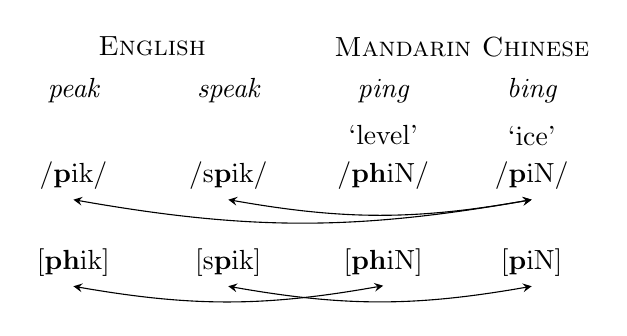
\begin{tikzpicture}[>=stealth, node distance=5mm and 1cm]
\node (peak_orth) {\itshape peak};
\node (speak_orth) [right = of peak_orth] {\itshape speak};
\node (ping_orth) [right = of speak_orth] {\itshape ping};
\node (bing_orth) [right = of ping_orth] {\itshape bing};
\node[xshift=1cm] (english) [above = 0.1\baselineskip of peak_orth] {\scshape English};
\node[xshift=1cm] (mandarin) [above = 0.1\baselineskip of ping_orth] {\scshape Mandarin Chinese};
\node (ping_gloss) [below = 0.1\baselineskip of ping_orth] {`level’};
\node (bing_gloss) [below = 0.1\baselineskip of bing_orth] {`ice’};
\node (peak_phoneme) [below = of peak_orth] {/\textipa{{\bfseries p}ik}/};
\node (speak_phoneme) [below = of speak_orth] {/\textipa{s{\bfseries p}ik}/};
\node (ping_phoneme) [below = of ping_orth] {/\textipa{{\bfseries p\super h}iN}/};
\node (bing_phoneme) [below = of bing_orth] {/\textipa{{\bfseries p}iN}/};
\node (peak_phone) [below = of peak_phoneme] {[\textipa{{\bfseries p\super h}ik}]};
\node (speak_phone) [below = of speak_phoneme] {[\textipa{s{\bfseries p}ik}]};
\node (ping_phone) [below = of ping_phoneme] {[\textipa{{\bfseries p\super h}iN}]};
\node (bing_phone) [below = of bing_phoneme] {[\textipa{{\bfseries p}iN}]};
\draw[<->] (peak_phoneme.south) to [bend right=10] (bing_phoneme.south);
\draw[<->] (speak_phoneme.south) to [bend right=10] (bing_phoneme.south);
\draw[<->] (peak_phone.south) to [bend right=10] (ping_phone.south);
\draw[<->] (speak_phone.south) to [bend right=10] (bing_phone.south);
\end{tikzpicture}
  \caption{Words, phonemes (slashes), and phones (square brackets).}
\label{example}
\end{figure}

Most multilingual acoustic models simply use existing phoneme transcriptions as-is, taking the union of the phoneme sets to be shared by all training languages \cite{lin2009study,cohen1997towards,schultz2001language,schultz1997fast,li2020zero}.
The assumption is reasonable under some circumstances as phoneme names are typically associated with their most common or least marked allophone. 
%\drm{Linguists would say ``least marked'' rather than ``simplest''. But really, phonemes are generally named after the allophone with the least restricted distribution.}.
However, this is obviously an over-simplistic view: in Figure \ref{example}, for example, this would mean that all training in English would assign the phones [\textipa{p}] and [\textipa{p\super h}] to phoneme /\textipa{p}/. This is detrimental if we want to recognize Mandarin Chinese, for instance, where the two phones are corresponding to two distinctive phonemes /\textipa{p}/ and /\textipa{p\super h}/.
% Therefore, merging phonemes to create a shared phoneme inventory would cause the degradation in performance. Additionally, a specific lexicon needs to be designed to adapt to the existing shared phoneme inventory when adding new languages, which adds much more works for linguists. Finally, phoneme transcriptions are typically broad transriptions, which might not be very useful for phoneticians.

%As of 2009, even Bible has just been translated into only 2508 languages~\cite{lewis2009ethnologue}.
%As a result, there is an increasing interest in building speech tools benefiting low resource languages. One promising tool for low resource language is the universal phone recognizer. A decent phone recognition system could play critical roles in a wide variety of other applications: endangered language documentation, creating speech synthesizers for language without standarized orthography, identifying language with language models \cite{matejka2005phonotactic}

%As collecting annotation for low resource languages is expensive and time-consuming, researchers have exploited data augmentation~\cite{ragni2014data, kanda2013elastic}, articulatory features~\cite{stuker2003integrating} and multilingual techniques \cite{schultz2001language, tong2017investigation, vu2013multilingual, tuske2013investigation, dalmia2018sequence}. 



%Most multilingual acoustic research based on the assumption that there exists a language dependent phoneme set to express phoneme of each languages. The assumption is reasonable under some circumstances as phonemes are usually associated with their underlying articulatory features which is mostly language dependent. However, there are several drawbacks of this approach: firstly, an identical phoneme might have different allophone realizations across languages, for instance, (give some examples here). Therefore, merging phonemes to create a shared phoneme inventory would cause the degradation in performance. Additionally, specific lexicon of each language has to be customized to adapt to the shared phoneme inventory, which adds much more works for linguists. Finally, phoneme transcriptions are typically broad transriptions, which might  not be very useful for phoneticians.

In this paper, we propose a novel method for multilingual recognition based on phonetic annotation to tackle this problem: \textit{Allosaurus} (\textbf{allo}phone \textbf{s}ystem of \textbf{au}tomatic \textbf{r}ecognition for \textbf{u}niversal \textbf{s}peech).
Our method incorporates knowledge of phonology into the multilingual model through an \textit{allophone layer}, which associates a universal narrow phone set with the phonemes that appear in the transcription of each language.
Our model first computes the phone distribution using a standard ASR encoder, then the allophone layer maps the phone distribution into the phoneme distribution for each language.
This model can be trained end-to-end using only standard phonemic transcriptions and an allophone list created by phoneticians.
The allophone layer is first initialized with the allophone list, then is further optimized during the training process.
We demonstrate that accounting for the phoneme-phone mismatch in this way improves the accuracy of multilingual acoustic modeling by 2.0\% phoneme error rate in low-resource conditions.

%In our experiment, our model equipped with the allophone layer is compared with the two standard models. We show that our model outpeform both groups in all of our testing languages.

Furthermore, the architecture simultaneously makes it possible to perform \emph{universal phone recognition}.
Previous approaches cannot perform phone recognition in a universal fashion as they depend on language-specific phonemes, as illustrated with the previous example of English not distinguishing /\textipa{p}/ and /\textipa{p \super h}/ as required in Mandarin.
% For example,  A model simply trained on English phoneme /\textipa{p}/ would not be able to distinguish Mandarin phoneme /\textipa{p}/ and /\textipa{p \super h}/.
In contrast, because our approach allows recognition of phones directly, it already has learned to make these fine-grained distinctions.
Taking advantage of this fact, we incorporate a large phone inventory database collected by linguists, PHOIBLE \cite{phoible}, and demonstrate that our phone recognizer can be customized to recognize over 2000 languages without any training data in the languages themselves.
By evaluating the recognizer with completely unseen testing languages, we found that our recognizer achieves 17\% better performance absolute compared with the traditional approach. 

%\gn{Need to be a little more explicit why this was not possible with previous methods.}

%By incorporating a large phone inventory database collected by linguists, PHOIBLE\cite{phoible}, we demonstrate that our phone recognizer can be customized to recognize over 2000 languages without any training data in the language.
%By evaluating the recognizer with unseen testing languages, we found that our recognizer achieves 20\%  better performance compared with the traditional approach.
% \gn{If you want to save space, I think the rest of the section can be commented out:}
% The contribution of this paper is two-fold:

% \begin{itemize}
%     \item We propose an architecture based on allophone layer, which explicitly incorporates knowledge from phonetics
%     \item Our model enables us to create an universal phone recognizer, which are further customized into more than 2000 language recognizers.
% \end{itemize}

\section{Related Work}
\label{sec:related}

While some recent work in multilingual ASR focuses on end-to-end models to directly predict graphemes~\cite{watanabe2017language, toshniwal2018multilingual}, most systems still depend on phonetically inspired acoustic models. Multilingual acoustic models fall into two groups.
The first group, \emph{shared phoneme} models, creates a shared phoneme inventory of all phonemes from all training languages~\cite{lin2009study,cohen1997towards,schultz2001language,schultz1997fast,li2020zero, thompson2019transferable}.
The second group, \emph{private phoneme} models, treats phonemes from each language as completely different classes performs phoneme classification separately for each language~\cite{huang2013cross,dalmia2018sequence,li2019multilingual}.
However, these two groups have their own respective drawbacks: the first group fails to consider the disconnect between the phonemes across languages while the second group completely ignores cross-lingual phonetic associations and is not applicable to recognition of new languages. In contrast, our approach solves both of these problems by taking into account allophones with phone-phoneme mappings.

There have been some attempts to apply phone recognizers to low resource languages. For example, English recognizers have been applied to align transcription corpora of an endangered language \cite{dicanio2013using}, facilitate language documentation \cite{michaud2018integrating}, identify languages with language models \cite{matejka2005phonotactic}, and perform linguistic annotation \cite{neubig2018towards}. However, these approaches depend heavily on training data in the language of interest and their specific phonemic transcriptions. Our approach, on the other hand, abstracts away the dependency to phonemes by applying the allophone transformations.

%Disadvange: dependency on monolingual or phonemeic transcription of training languages


%several groups depending on its targets' granularity. For instance, the network can be trained to predict the language independent grapheme~\cite{watanabe2017language, toshniwal2018multilingual}

%Multilingual speech recognition has explored various methods to share parameters across languages in different ways.
%For example, parameters can be shared by using posterior features from other languages \cite{stolcke2006cross}, applying the same GMM components across different HMM states \cite{burget2010multilingual}, training shared hidden layers in DNNs \cite{huang2013cross, heigold2013multilingual,dalmia2018sequence}, or using language independent bottleneck features \cite{thang:sltu2012, dalmia2018domain}.

%Multilingual acoustic modeling can be divided into several groups depending on its targets' granularity. For instance, the network can be trained to predict the language independent grapheme~\cite{watanabe2017language, toshniwal2018multilingual}. These methods fall into two groups: the first group creates a shared phoneme inventory by merging phonemes from all training languages~\cite{lin2009study,cohen1997towards,schultz2001language,schultz1997fast,li2018zero}, while the second group treats phonemes from each language as completely different classes and applies a language dependent layer to classify phonemes for each language~\cite{huang2013cross,dalmia2018sequence}. We refer to this type of model as the private phoneme model in the following section. However, these two groups have their own respective drawbacks: the first group fails to consider the disconnect between the phonemes across languages while the second group completely ignores cross-lingual phonetic associations and is not applicable to recognition of new languages. In contrast, our approach solves both of these problems by taking account of allophones with phone-phoneme mappings.

%\gn{This paragraph seems important, but it's pretty vague and hard to follow. Can you take another look and try to fix to be more clear?}\xj{TODO: rewrite this paragraph}

%On top of those multilingual recognition works, there has been attempts to build phone recognizers across languages: combining multilingual acoustic model by applying polyphone decision trees to GlobalPhone inventory \cite{schultz1998language}. Constructing phoneme associations by using similarity over gaussian distributions \cite{kumar2005multilingual}. However, most works only develop the broad phoneme-level recognition. On the contrary, this work focuses on the narrow phone-level recognition. \drm{I do not understand this paragraph, so I agree with GN that you should revise it.}

%Some models only share their hidden layers, but use separate output layers to predict their phones \cite{huang2013cross, heigold2013multilingual}. Other models have only one shared output layer to predict the universal phone set shared by all languages \cite{schultz2001language, tong2017investigation, vu2013multilingual}. 

%While those works proposed the multilingual models in different ways, few of them have explicitly exploited the relatedness across various languages and corpora. In contrast, our work computes the relatedness between different corpora using the embedding representations and exploits them efficiently.

%The multilingual architecture so far falls into two groups: the first group is to treat phonemes from different languages as identical groups, then create a universal phoneme set by merging them together; the second group treat phonemes from each language as completely different classes, then apply a language dependent layer to classify phonemes for each language. However, those two groups have their own drawbacks respectively: the first group fails to consider phone realization in each language, for example, blablabla. The second group ignore the association between phonemes across different languages.

%Multilingual acoustic modeling has been successfully applied to low resource languages. Most research so far can be divided into two groups: the first group 


%ocused on recognizing either language dependent phonemes \cite{huang2013cross}

%There has been attempts to build phone recognizers across languages: combining multilingual acoustic model by applying polyphone decision trees to GlobalPhone inventory \cite{schultz1998language}. Constructing phoneme associations by using similarity over gaussian distributions \cite{kumar2005multilingual}

%In addition to the usage of speech recognition and speech synthesizers, a decent phone recognition could play critical roles in a wide variety of other applications: endangered language documentation, creating speech synthesizers for language without standarized orthography, identifying language with language models \cite{matejka2005phonotactic}

%One typical line of work is to separate the model into acoustic model and language model (some citations here), where parameters across language can be shared in the acoustic model. 


\section{Approach}
%In this section, we describe the proposed architecture as well as the baseline architecture. 

\begin{figure}[t]
  \centering
  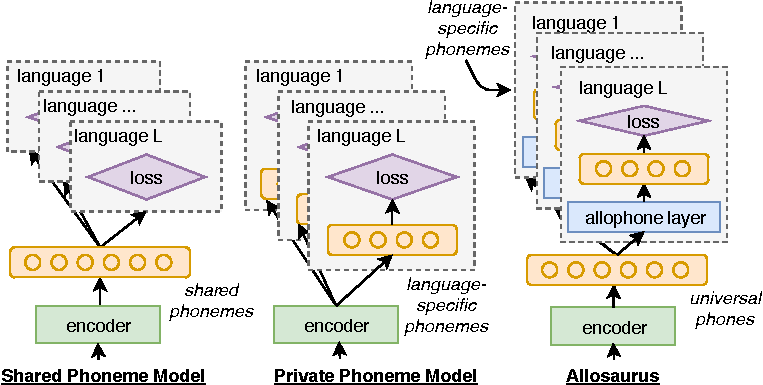
\includegraphics[width=\columnwidth]{allosaurus.pdf}
  \caption{Traditional approaches predict phonemes directly, either for all languages (left) or separately for each language (middle). On the contrary, our approach (right) predicts over a shared phone inventory, then maps into language-specific phonemes with an allophone layer.}
  \vspace{-3mm}
\label{arch}
\end{figure}

\subsection{Phone-Phoneme Annotation}
% Unlike previous works in multilingual speech recognition, phones and phonemes are explicitly distinguished in this work.
Suppose there are $|L|$ training languages, and each language $L_i$ has its own phoneme inventory $Q_{i}$ which can be easily obtained by enumerating the phonemes appearing in its annotated training data.
Most traditional multilingual approaches handle inventories at the phoneme level, and create a \textit{shared phoneme inventory} $Q_{\text{sha}}$ by taking union of the phoneme sets:

\begin{equation}
    \small
    Q_{\text{sha}} = \bigcup_{1 \leq i \leq |L| } Q_i.
\end{equation}

% This approach, however, fails to capture the realizations of phonemes in each language. 
In contrast, our method distinguishes phonemes from their phone realizations.
We have linguists annotate each phoneme $q \in Q_{i}$ with its corresponding allophone set $P^i_q$, where each phone $p \in P^i_q$ is a realization of $q$ in language $L_i$.
%For instance, the English phoneme $/k/$ has two phone realizations: $\{ [k], [k^h] \}$ \gn{This sentence could be removed if it's already clearly stated in the intro.}. \drm{Since this is effectively the same example as in the intro, it seems redundant here}.
Merging these sets for all languages, we obtain the \textit{universal phone inventory} $P_{\text{uni}}$.

\begin{equation}
    \small
    P_{\text{uni}} = \bigcup_{1 \leq i \leq |L| } \bigcup_{q \in Q_{i}} P^i_q
\end{equation}

Additionally, we obtain a \textit{signature matrix} $S^i = \{0, 1\}^{|Q_i| \times |P_{\text{uni}}|} $ describing the association of phone and phonemes in each language $L_i$: Suppose the phoneme $q \in Q_i$ has the row index $j$ where $1 \leq j \leq |Q_i|$ , phone $p \in P_{\text{uni}}$ has the column index $k$ where $1 \leq k \leq |P_{\text{uni}}|$, if the $p$ is a realization of $q$, then $(j,k)$ cell of the $S^i$ has a value of 1, otherwise it is assigned 0.

%the association of whether phoneme $q$ has phone $p$ in its allophone set in each language $L_i$ 
%\drm{Something here is not idiomatic English but I'm not sure exactly what you mean, so I can't fix it}. 
%The corresponding $({p,q})$ cell in the matrix is 1 if there exists the allophone relationship, otherwise, 0 is assigned.

\subsection{Allophone Layer}

%Equipped with the universal phone inventory $P_{uni}$ and the signature matrix $\mathcal{S}^i_{p,q}$, 
%Our model establishe between phone and phonemes by using the allophone layer. 
As mentioned in Section~\ref{sec:related}, traditional multilingual models can be divided into two groups.
The first group, \emph{shared phoneme models} (Figure \ref{arch} left), predicts phoneme distributions over the shared phoneme inventory $Q_{\text{sha}}$. The second group, \emph{private phoneme models} (Figure \ref{arch} middle), on the other hand, shares a common encoder but computes distribution over private phoneme inventory $Q_i$ for each language $L_i$. These approaches handle phonemes directly with no concept of underlying phones.

\begin{table*}[t!]
\begin{center}
    \caption{Results of three models' phoneme error rate performance on 11 languages. The top-half shows the results trained with all training datasets. The bottom-half shows the low-resource results in which only 1k utterances are used for training from each dataset.} \label{tab:training_results} %\gn{Make the best number bold in each column for both the top and bottom sections.}} \label{tab:training_results}
    %\gn{You need to explain what he difference between the top results and bottom results are in the caption, and also hopefully add a label to the left side of the two sections.}} \label{tab:training_results}
    \begin{tabular}{l l | c c c c c c c c c c c | c} 
    \toprule
    & & Amh & Eng & Ger & Ita & Jap & Man & Rus & Spa & Tag & Tur & Vie & Average \\
    \midrule
    \multirow{3}{*}{\rotatebox{90}{\textbf{Full}}} & \textbf{Shared Phoneme PER}  & 78.4 & 71.7 & 71.6 & 62.9 & 65.9 & 76.5 & 76.9 & 62.6 & 74.1 & 76.6 & 82.7 & 73.8 \\
    & \textbf{Private Phoneme PER} & 37.1 & 22.4 & 17.6 & 26.2 & 17.6 & 17.9 & 21.3 & 18.5 & 47.6 & 35.8 & 56.5 & 25.6 \\
    & \textbf{Allosaurus PER} & 36.0 & 20.5 & 18.8 & 23.7 & 23.8 & 17.0 & 26.3 & 19.4 & 57.4 & 35.3 & 57.3 & 25.0 \\
    \midrule
    \multirow{3}{*}{\rotatebox{90}{\textbf{Low}}} & \textbf{Shared Phoneme PER} & 80.4 & 73.3 & 74.3 & 72.2  & 77.1 & 83.0 & 83.2 & 72.8 & 84.8 & 84.4 & 84.5 & 78.4 \\
    & \textbf{Private Phoneme PER} & 55.4 & 50.6 & 41.9 & 31.6 & 36.8 & 37.0 & 47.9 & 36.7 & 62.3 & 54.5 & 73.6 & 43.8 \\
    & \textbf{Allosaurus PER} & 54.8 & 47.0 & 41.5 & 37.4 & 40.5 & 33.4 & 45.0 & 35.9 & 70.1 & 53.6 & 72.5 & 41.8 \\
    \bottomrule
    \end{tabular}
    \vspace{-2mm}
\end{center}
\end{table*}


\begin{table}[t!]
\begin{center}
    \caption{Training corpora and size in utterances for each language. Models are trained and tested with 12 rich resource languages (top) and 2 low resource unseen languages (bottom).} \label{tab:corpus}
    \resizebox{\columnwidth}{!}{
    \begin{tabular}{l l r} 
    \toprule
    {\bf Language} & {\bf Corpora} & {\bf Utt.} \\
    \midrule
    English & voxforge, Tedlium \cite{rousseau2012ted}, Switchboard \cite{godfrey1992switchboard} & 1148k \\
    Japanese & Japanese CSJ \cite{maekawa2003corpus} &  440k \\
    Mandarin & Hkust \cite{liu2006hkust}, openSLR \cite{aishell_2017,THCHS30_2015} & 377k \\
    Tagalog & IARPA-babel106b-v0.2g & 93k \\
    Turkish & IARPA-babel105b-v0.4 & 82k \\
    Vietnamese & IARPA-babel107b-v0.7 & 79k \\
    German & voxforge & 40k \\
    Spanish & LDC2002S25 & 32k \\
    Amharic & openSLR25 \cite{Abate2005} & 10k \\
    Italian & voxforge & 10k \\
    Russian & voxforge & 8k \\
    \midrule
    Inukitut & private & 1k \\
    Tusom & private & 1k \\
    %Amharic & LDC2014S06 (babel) & telephone & 41,403 & Bengali & LDC2016S08 (babel) & telephone & 60,663 \\
    %Dutch & voxforge (vox) & read  & 8,492 & German & voxforge (vox) & read & 41,146 \\
    %Spanish & LDC98S74 (hub) & broadcast & 31,615 & Swahili & LDC2017S05(babel) & telephone & 44,502 \\
    %Turkish & LDC2012S06 (hub) \cite{saraclar2012turkish} & broadcast & 97,427 & Zulu & LDC2017S19 (babel) & telephone & 60,835 \\
    \bottomrule
    \end{tabular}
    }
    \vspace{-2mm}
\end{center}
\end{table}
%The logits $l_q$ are further connected with loss function in each language.


In contrast our proposed approach, \emph{Allosaurus},  (Figure \ref{arch} right), comprises a language independent encoder and phone predictor, and a language dependent allophone layer and a loss function associated with each language. The encoder first produces the distribution $h \in \mathbb{R}^{|P_{\text{uni}}|}$ over the universal phone inventory $P_{\text{uni}}$, then the allophone layer transforms $h$ into phoneme distribution $g^i \in \mathbb{R}^{|Q_{i}|}$ of each language. 
The allophone layer uses a trainable allophone matrix $W^i \in \mathbb{R}^{|Q_i| \times |P_{\text{uni}}|}$ to describe allophones in the similar way as $S^i$. The allophone matrix $W^i$ is first initialized with $S^i$, and is allowed to be optimized during the training process, but we add an L2 penalty to penalize divergence from the original signature matrix $S^i$. The allophone layer computes its logit distribution $g^i$ by finding the most likely allophone realization in $P_{\text{uni}}$ with maxpooling. %\gn{I couldn't understand the following equation...}

%Unlike previous works in multilingual acoustic modeling, we explicitly model the phone distribution from the encoder: each dimension in the phone distribution outputs is corresponding exactly to an narrow phone. 

%In this paper, we propose two different allophone layers for our architecture: linear allophone layer and pooling allophone layer.

%\textbf{linear allophone} models the phone-phoneme mapping linearly. Suppose the $p_{narrow}$ represents the distribution over phones and $p_{broad}$ represents the distribution over phonemes. The linear allophone layer estimate the distribution as follows:

%\begin{equation}
%l_{q}=\sum_{p \in p^i_q} h_{p}
%\end{equation}

%\textbf{pooling allophone} improves the linear architecture by selecting one phone from %allophones. 

\begin{equation}
g^i_{j}=\max(\{ w^i_{j,k} \cdot h_{k} ; 1 \leq k \leq |P_{\text{uni}}| \}),
\end{equation}
where $g^i_{j} \in \mathbb{R}$ is the logit of $j$-th phoneme in $g^i$ for language $L_i$, $w^i_{j,k} \in \mathbb{R}$ is the $(j,k)$ cell of the allophone matrix $W^i$, $h_{k} \in \mathbb{R}$ is the logit of $k$-th phone in $h$. Intuitively, if the $j$-th phoneme has the $k$-th phone as an allophone, $w^i_{j,k}$ would be near 1, otherwise $w^i_{j,k}$ would be near 0. Therefore, the phoneme logit of $g^i_j$ is decided by the largest allophone logit $h_k$. The phoneme distribution $g^i$ is further fed into the loss function. This method for phoneme prediction can be used with any underlying multilingual ASR system. Here we specifically optimize the parameters by minimizing CTC loss \cite{graves2006connectionist} for all training languages, with the addition of regularization of the allophone layer controlled by hyperparameter $\alpha$. %Increasing $\alpha$ might help the model to learn cleaner representations of phones, but the allophone layer is less likely to be adapted to the phonemes in the training set.

%Add interpretation of previous regularization under Bayesian informative prior. Maybe LASSO instead of ridge to improve sparsity?

\begin{equation}
\mathcal{L}=\sum_{1 \leq i \leq |L|} (\mathcal{L}^i_{ctc} + \alpha \norm{ W^i-S^i }_2^2 ).
\vspace{-2mm}
\end{equation}


\subsection{Universal Phone Recognition}
%Not only the allophone layer solves the \textit{phoneme compatibility} issue by inserting the allophone layer, which contributes to the improvement in the multilingual acoustic modeling. More importantly, the model endows us with the capability to predict universal narrow phones explicitly, which was rarely attempted by previous works.

Not only does the allophone layer abstract away from the language-specific phonemes, which contributes to the improvement in the multilingual acoustic modeling, the model also gives us the capability to predict universal phones themselves.
This has rarely been attempted in previous work.
By applying the greedy decoding strategy over the phone distribution $h$, we can obtain a phone sequence in which all phones $P_{\text{uni}}$ in the training languages are candidates. When combined with a large training languages sets, our universal inventory is expected to cover most common narrow phones appearing in many languages in the world, which we show in the experiment section. 

Furthermore, this recognition protocol can take into account phone inventories that have already been created for many languages in the world by linguists.
For example, PHOIBLE \cite{phoible} is a database of phone inventories for more than 2000 languages and dialects, allowing our model to be applied to these languages with some degree of accuracy.
If the phone inventory for language $L_i$ is $P_i$, we can restrict the decoder to only produce phones in $P_i \cap P_{\text{uni}}$ by filtering out other phones.
When the universal inventory $P_{\text{uni}}$ covers most frequent phones in the world, we could expect that $P_i \approx P_i \cap P_{\text{uni}}$.%, which means our model could recognize most phones in the target language.

%\subsection{Phone Remapping}
%We map phone with panphon distance.

%\subsection{Universal Prior Compensation}
%To compensate for the imbalanced phone distribution in the training set, we introduce the phone prior compensation for the recognition \cite{bishop2006pattern}.

%\begin{equation}
%\mathbb{P}(p|\mathbf{x}) = %\frac{\mathbb{P}(p|\mathbf{x})}{\mathbb{P}_\mathcal{D}(p)} %\mathbb{P}_{world}(p)
%\end{equation}

%where the $\mathbb{P}_{\mathcal{D}}(p)$ is the phone prior in the training data, and $\mathbb{P}_{world}(p)$ is the phone prior in languages universally.

\section{Experiments}

\subsection{Settings}
As we are interested in creating a large universal phone inventory, we select a phonetically diverse set of 11 training languages as summarized on the top of Table~\ref{tab:corpus}. We include corpora from a variety of speech domains to make our model robust (e.g., read speech, sponatenuous speech). 5\% of the dataset is used as the test set, and the remaining data are used as the training set and the validation set. We also consider a low resource condition, where 1,000 random utterances are used from each corpus to train the model. As baselines, we compare with the previously-described \textit{shared phoneme} and \textit{private phoneme} models.
All methods use the same encoder and features.
Features are high-resolution 40 dimensional MFCCs extracted with Kaldi~\cite{povey2011kaldi}. The encoder is a 6-layer stacked bidirectional LSTM with hidden size of 1024 in each layer. The regularization hyperparameter $\alpha$ is set to 10.
Phonemes for training languages are assigned using the grapheme-to-phoneme tool Epitran \cite{mortensen2018epitran}.
%.\drm{I would prefer that Epitran was not identified as ours and was cited, but I don't know the ICASSP anonymity rules.} 
For each phoneme in each language, phoneticians (mostly authors of this paper) create the allophone mappings.\footnote{This work has been accepted to LREC 2020 and its database is available at \url{https://github.com/dmort27/allovera}}

We evaluate using phoneme error rate for the training languages.
Furthermore, we select two languages not included in the training data: Inukitut and Tusom.
These languages are indigenous languages with few training resources, representing a realistic scenario where our model is applied to entirely new languages, as may be done when ASR is used for documentation of endangered languages.
The datasets of these two languages are transcribed with phones, and accordingly we use phone error rate rather than the phoneme error rate.
While Allosaurus is able to predict phones in a natural way by decoding $h$, the two baselines could not predict phones directly. In this unseen language experiment, we assume phonemes predicted by the baselines correspond to phones of the same name.


%For the testing languages (Inukitut, Tusom).

%Previous multilingual models were typically trained with GlobalPhone %\cite{schultz2002globalphone}. In contrast, our datasets contain 10x larger utterances and %speakers.

%\subsection{Settings}
%We implement both allophone acoustic models proposed above and contrasts it with the baseline model. The encoder is a 6-layer stacked bidirectional LSTM with 1024 hidden size in each layer. Phonemes of each language are assigned using our orthography tool: epitran. For each phoneme in each language, phoneticians create the allophone mappings.

% \begin{table*}[t]
% \begin{center}
%     \caption{Statistics of the phone coverage mean (standard deviation) of language families and areas ranked by the number of languages. Phone coverage of language $L_i$ is defined as $\frac{| P_{\text{uni}} \cap P_{i}|}{|P_{i}|}$} \label{tab:family}
%     \begin{tabular}{l r r r | l r r r} 
%     \toprule
%     {\bf Area} & {\bf \# Language} & {\bf Shared} & {\bf Allosaurus} & {\bf Family} & {\bf \# Language }  & {\bf Shared} & {\bf Allosaurus}\\
%     \midrule
%      Africa & 875 & 53\% (13\%)&  84\% (11\%) & Bantoid & 235 & 55\% (12\%) & 87\% (10\%)\\
%      America & 659 & 52\% (14\%) & 81\% (13\%) & Arawakan & 65 & 56\% (12\%) & 88\% (8\%)  \\
%     Asia & 377 & 46\% (15\%) & 79\% (13\%) & Kwa & 63 & 54\% (12\%) & 82\% (10\%) \\
%     Pacific & 152 & 59\% (15\%) & 87\% (12\%) & Gur & 60 & 57\% (13\%) & 85\% (9\%) \\
%     Europe & 92 & 35\% (9.5\%) & 69\% (13\%)  & Tupi-Guaraní & 46 & 56\% (12\%) & 86\% (7.9\%) \\
%     \midrule
%     All & 2155 & 52\% (15\%) & 82\% (13\%) & All & 2155 & 52\% (15\%) & 82\% (13\%) \\

%     %& Indic & 45 & 0.322(0.092) & 0.664(0.105) \\
%     %Oceanic & 39 & 0.596(0.167) & 0.885 (0.102) & Western Mande & 38 & 0.569(0.106) & 0.872(0.071) \\
%     %Cariban & 37 & 0.580(0.113) & 0.898(0.067) & Biu-Mandara & 36 & 0.568(0.072) & 0.856(0.066) \\
%     \bottomrule
%     \end{tabular}
%     \vspace{-2mm}
% \end{center}
% \end{table*}


\begin{table}[t]
\begin{center}
    \caption{Statistics of the phone coverage mean (standard deviation) of areas. Phone coverage of language $L_i$ is defined as $\frac{| P_{\text{uni}} \cap P_{i}|}{|P_{i}|}$} \label{tab:family}
    \begin{tabular}{l r r r } 
    \toprule
    {\bf Area} & {\bf \# Language} & {\bf Shared} & {\bf Allosaurus} \\
    \midrule
     Africa & 875 & 53\% (13\%)&  84\% (11\%) \\
     America & 659 & 52\% (14\%) & 81\% (13\%) \\
    Asia & 377 & 46\% (15\%) & 79\% (13\%) \\
    Pacific & 152 & 59\% (15\%) & 87\% (12\%) \\
    Europe & 92 & 35\% (9.5\%) & 69\% (13\%) \\
    \midrule
    All & 2155 & 52\% (15\%) & 82\% (13\%) \\

    %& Indic & 45 & 0.322(0.092) & 0.664(0.105) \\
    %Oceanic & 39 & 0.596(0.167) & 0.885 (0.102) & Western Mande & 38 & 0.569(0.106) & 0.872(0.071) \\
    %Cariban & 37 & 0.580(0.113) & 0.898(0.067) & Biu-Mandara & 36 & 0.568(0.072) & 0.856(0.066) \\
    \bottomrule
    \end{tabular}
    \vspace{-2mm}
\end{center}
\end{table}

\begin{table}[t]
\begin{center}
    \caption{Comparisons of phone error rates in two unseen languages} \label{tab:unseen_results}
    %\drm{Shouldn't the pluses go {\bfseries after} the numbers? And do you explain why PHOIBLE is in parentheses? And why don't we have exact values for Allosaurus+PHOIBLE?}}
    %some numbers are still placeholder, need to be updated
    %\label{tab:unseen_results}
    \begin{tabular}{l r r} 
    \toprule
    & Inuktitut & Tusom \\
    \midrule
    \textbf{Shared Phoneme PER} & 94.1 & 93.5 \\
    \textbf{Best Private Phoneme PER} & 86.2 & 85.8 \\
    %\textbf{Private Mandarin} & & \\
    \midrule
    \textbf{Allosaurus PER} & 84.1 & 77.3  \\
    \textbf{Allosaurus+PHOIBLE PER} & 73.1 & 64.2 \\
    \bottomrule
    \end{tabular}
    \vspace{-2mm}
\end{center}
\end{table}

\subsection{Main Results}

% point in this section
% - Allosaurus is comparable with the Private Phoneme model
% - Private phoneme model is better than the shared phoneme model

Table~\ref{tab:training_results} demonstrates the performance of the baseline models and Allosaurus evaluated on 11 languages. The top half of the table summarizes the performance when trained with the full training set. The results suggests both the private phoneme model and the Allosaurus model outperforms the shared phoneme model significantly. The results of the shared phoneme model can be explained by the disagreement of phoneme assignments across languages. In contrast, the private phoneme model handles this issue by using language specific phoneme layers. Our model also circumvents this issue by introducing the language-specific allophone layers. The bottom half of the Table~\ref{tab:training_results} highlights the results when the training set of each language is limited as mentioned above. Unsurprisingly, limiting the amount of training data hurts accuracy across the board. While the private phoneme model and our model achieve similar results when using the full training set, our model outperforms the private phoneme model by 2.0\% when training data is limited. This suggests that our model is better at sharing parameters across languages by using prior phonetic knowledge in this case, likely due to the fact that the private phoneme model needs to learn each phoneme predictor from scratch, while our model already has phone-phoneme mapping knowledge seeded by linguistically motivated annotations.

\begin{table}[t]
\begin{center}
    \caption{An English example from switchboard in which Allosaurus could distinguish [\textipa{p\super h}] and [\textipa{p}] for phoneme /\textipa{p}/} \label{tab:english_res}
    %\drm{Shouldn't the pluses go {\bfseries after} the numbers? And do you explain why PHOIBLE is in parentheses? And why don't we have exact values for Allosaurus+PHOIBLE?}}
    %some numbers are still placeholder, need to be updated
    %\label{tab:unseen_results}
    \begin{tabular}{l l} 
    \toprule
    Model & Phones  \\
    \midrule
    \textbf{Utterance} & the quebec \textbf{people} that that \textbf{speak} french \\
    \textbf{Annotation} & /\dh \, \textipa{@} \textipa{k} \textipa{w} \textipa{@} b \textipa{E} k \textbf{\textipa{p}} \textipa{i} \textipa{p} \textipa{@} \textipa{l} .. \textipa{s} \textbf{\textipa{p}} \textipa{i} \textipa{k} \textipa{f} \textturnr\, \textipa{E} \textipa{n} \textteshlig/ \\
    \textbf{Allosaurus} & [\dh \, \textipa{@} \textipa{x} \textipa{o} \textipa{b} \textipa{@} \textipa{k} \textturna \,
 \textbf{\textipa{p\super h}} \textipa{i} \texttheta\, \textipa{o:} \textipa{l} .. s \textbf{p} \textturnr\, \textipa{I} \textipa{k} \textipa{f} \textturnr\, \textipa{E} \textipa{n} \textipa{d}] \\
    \bottomrule
    \end{tabular}
    \vspace{-2mm}
\end{center}
\end{table}

%Unsuprisigly, the shared phoneme model still has difficulty 

%The table shows that the Allosaurus model outperforms the shared phoneme model significantly. On average, our Allosaurus model achieves 30\% better phoneme error rate compared with the shared phoneme model. On the other hand, the private phoneme model has similar performance as the Allosaurus model with respect to both PER and WER. 

\subsection{Universal Phone Recognition Results}

In addition to the improvements over low resource settings, our model enables us to predict (nearly-)universal phone distributions.
By merging phone inventories from all of our languages, we obtain a shared inventory of 187 phones. First, we assess how close this inventory gets to covering the languages registered in PHOIBLE.
%We define phone coverage of language $L_i$ is defined as $\frac{| P_{\text{uni}} \cap P_{i}|}{|P_{i}|}$.
The Allosaurus column in Table~\ref{tab:family} summarizes the phone coverage of our model, split into different geographic areas.
The phone coverage in each cell represents the mean and standard deviation for each category. As the table suggests, our model has a promising phone coverage over all areas consistently. On average, it has 82\% mean phone coverage and 12.8\% standard deviation over all PHOIBLE languages.
Furthermore, by comparing our model with the baseline model in which we merged all the phoneme inventories from the corpus as-is, we significantly improve the phone coverage by 30\%. Additionally, the standard deviation shows that our model covers phones more consistently than the baseline model.
%Further, in Table~\ref{tab:family} we list the top-5 language families in PHOIBLE ranked by the number of its languages.
%While these families contain a variety of low resource languages, the table indicates that our model can achieve high coverage across these families consistently as well.

Next, we actually evaluate the model with respect to its ability to recognize phones. Table \ref{tab:english_res} shows a decoded English example. The utterance contains three English phonemes /p/ in word \textit{people} and \textit{speak}. The underlying allophones, however, are [\textipa{p\super h}] and [\textipa{p}] as mentioned in Section 1. While the original English training set annotates those two words with the same phoneme /p/, Allosaurus is able to predict different allophones by leveraging knowledge from other languages (e.g: Mandarin). We also note that Allosaurus is still not perfect: it fails to recognize the second /p/ in ``people.''

Additionally we also investigate unseen languages on the Inuktitut and Tusom datasets. The results are summarized in the Table~\ref{tab:unseen_results}. As the result show, the shared phoneme model can hardly recognize any phonemes in these two languages, with more than 90.0\% phone error rate on both datasets.
Next, we try all 11 private phoneme models from the training datasets and use the one with the lowest phoneme error rate. %\gn{Please check that my interpretation here is correct.}.
Unsurprisingly, this also can not achieve satisfying results on both datasets, as none of our 11 languages is similar to Inuktitut and Tusom; they both have over 85.0\% phone error rate.
On the other hand, the proposed Allosaurus model achieves 84.1\% phone error rate on Inuktitut and 77.3\% phone error rate on Tusom, a significant drop.
When combined with the PHOIBLE inventory, the error rates are further improved to 73.1\% and 64.2\% respectively, which shows 17\% improvements on average over the shared phoneme baseline. Table \ref{tab:inuktitut_res} shows one qualitative example from Inuktitut data. It suggests that simply applying Allosaurus could capture some aspects of the target phonemes, but it still made many errors especially substitution errors between [e] and [i]. The reason is Allosaurus has a much broader phone search space (187 phones), it might be difficult to distinguish similar phones (e.g: both [e] and [i] are front vowels, but [e] is a close vowel and [i] is a close-mid vowel). We find those substitution errors account for the majority of errors in the test sets. Those confusing phones, however, might be solved when combined with an appropriate inventory such as PHOIBLE. The last row suggests that Allosaurus could fix those substitution errors as [e] does not exist in Inuktitut's inventory. %The table also suggests Allosaurus is able to learn rare phones from relatively small samples. For example, the phone [\textipa{l:}] is predicted correctly and it only appears in the Italian training set, which has very limited utterances.

%\xj{Discussion of actual results.}

\begin{table}[t]
\begin{center}
    \caption{A qualitative example from Inuktitut dataset} \label{tab:inuktitut_res}
    %\drm{Shouldn't the pluses go {\bfseries after} the numbers? And do you explain why PHOIBLE is in parentheses? And why don't we have exact values for Allosaurus+PHOIBLE?}}
    %some numbers are still placeholder, need to be updated
    %\label{tab:unseen_results}
    \begin{tabular}{l l} 
    \toprule
    Model & Phones  \\
    \midrule
    \textbf{Ground Truth} & [\textipa{i} \textipa{l} \textipa{i} \textipa{t} \textipa{s} \textipa{i} \textipa{l:} \textipa{i}] \\
    \textbf{Allosaurus} & [\textipa{e} \textipa{l} \textipa{e} \textipa{p} \textscr\, \textipa{I} \textipa{l:} \textipa{e}] \\
    \textbf{Allosaurus+PHOIBLE} & [\textipa{i} \textipa{l} \textipa{i} \textipa{t} \textipa{i} \textipa{l:} \textipa{i:}] \\
    \bottomrule
    \end{tabular}
    \vspace{-2mm}
\end{center}
\end{table}

%(I will add some discussion here)

\section{Conclusion}
In this work, we propose \textit{Allosaurus}, which considers the relationship between phones and phonemes in multilingual acoustic modeling. %The model has improved the accuracy of baseline multilingual ASR methods by 2.0\% over 11 training languages. Furthermore, 
It improves significantly the phone recognition accuracy over unseen languages by 17\%.

\section{Acknowledgment}
This work is supported by NSF awards ACI-1548562 and 1761548. We would like to thank Alexis Michaud, Steven Abney, Hilaria Cruz and other participants of the LTLDR workshop for their feedback.


%The private phoneme model







%to compare with all languages registered in 
    
%The inventory has a 

%Similarly, we merge all the phoneme inventories to compare as our baseline.




%show some statistics of evaluation.

%To demonstrate that the universal recognizer is helpful 

% \begin{table*}[t]
% \begin{center}
%     \caption{Statistics of phone coverage of language family ranked by the number of language} \label{tab:family}
%     \begin{tabular}{c c c c | c c c c} 
%     \toprule
%     {\bf Family} & {\bf \# Language} & {\bf Baseline} & {\bf Universal} & {\bf Family} & {\bf \# Language }  & {\bf Baseline} & {\bf Universal}\\
%     \midrule
%     Bantoid & 235 & 0.558(0.129) & 0.872 (0.102) & Arawakan & 65 & 0.564(0.129) & 0.884(0.084) \\
%     Kwa & 63 &0.538(0.115) & 0.816 (0.095) & Gur & 60 &0.571(0.126) & 0.851(0.090) \\
%     Tupi-Guaraní & 46 &0.561(0.118) & 0.864(0.079) & Indic & 45 & 0.322(0.092) & 0.664(0.105) \\
%     Oceanic & 39 & 0.596(0.167) & 0.885 (0.102) & Western Mande & 38 & 0.569(0.106) & 0.872(0.071) \\
%     Cariban & 37 & 0.580(0.113) & 0.898(0.067) & Biu-Mandara & 36 & 0.568(0.072) & 0.856(0.066) \\
%     \bottomrule
%     \end{tabular}
% \end{center}
% \end{table*}

% \begin{table*}[h]
% \begin{center}
%     \caption{Statistics of phone coverage of language family ranked by the number of language} \label{tab:area}
%     \begin{tabular}{c c c c}
%     \toprule
%     {\bf Area} & {\bf \# Language} & {\bf Baseline} & {\bf Universal} \\
%     \midrule
%     Africa & 875 & 0.536(0.132) & 0.843(0.112)\\
%     America & 659 & 0.528(0.146) & 0.813(0.134)\\
%     Asia & 377 & 0.466(0.157) & 0.790(0.129)\\
%     Pacific & 152 & 0.590(0.151) &0.869(0.117) \\
%     Europe & 92 & 0.350(0.095) & 0.690(0.131) \\
%     \midrule
%     All & 2155 & 0.516(0.149) & 0.820(0.128) \\
%     \bottomrule
%     \end{tabular}
% \end{center}
% \end{table*}

%\section{Conclusion}

% References should be produced using the bibtex program from suitable
% BiBTeX files (here: strings, refs, manuals). The IEEEbib.bst bibliography
% style file from IEEE produces unsorted bibliography list.
% -------------------------------------------------------------------------
\bibliographystyle{IEEEbib}
\bibliography{refs}

\end{document}
